\label{sec:data}

\begin{wrapfigure}{r}{0.5\textwidth}
    \centering
    \vspace{-0.5cm}
    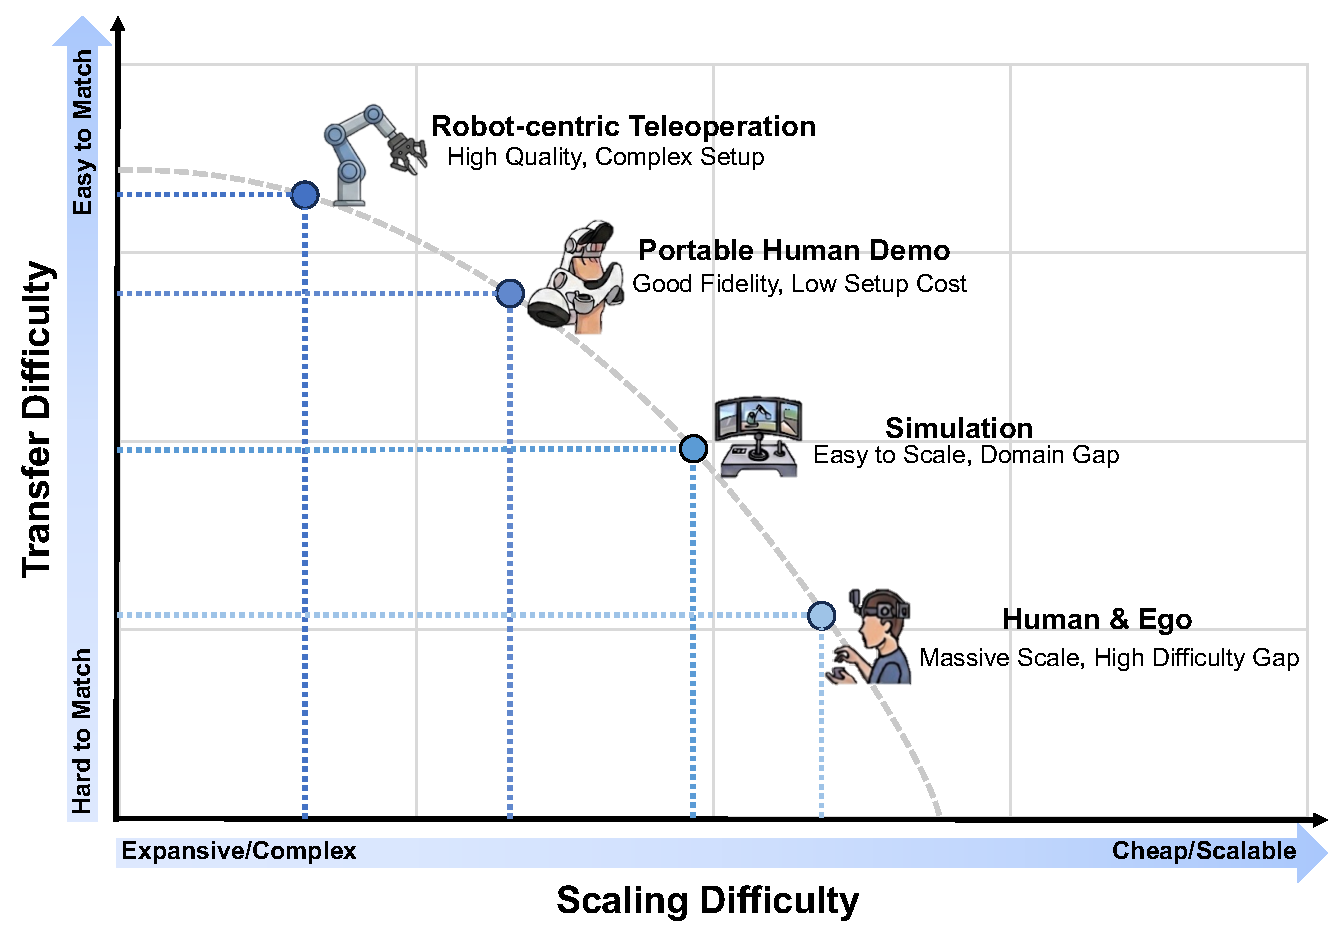
\includegraphics[width=\linewidth]{pic/data_overview.pdf}
    \vspace{-0.5cm}
    \caption{An overview of the embodied data landscape for training World Action Models, mapped across Transfer Difficulty (Y-axis) and Scaling Difficulty (X-axis).}
    \label{fig:data_overview}
    \vspace{-1cm}
\end{wrapfigure}


Training robust and generalizable World Action Models (WAMs) is fundamentally bottlenecked by the availability and quality of embodied data. Unlike large language models that thrive on passively scraped internet text, WAMs require strict physical grounding to capture complex state transitions, action conditioning, and intuitive physics. More importantly, the data requirements for WAMs diverge significantly from traditional robotic paradigms. Standard Vision-Language-Action (VLA) models strictly require paired $(o_t, a_t)$ trajectories, which severely restricts scalability given the high cost and scarcity of teleoperated demonstrations. Conversely, pure World Models thrive on action-free $(o_t, o_{t+1})$ sequences from internet videos but lack grounding in physical control. 



The unique advantage of WAMs lies in their \textbf{unified data digestion}. They uniquely benefit from the intersection of these domains, leveraging high-quality $(o_t, a_t, o_{t+1})$ triplets to tightly couple their internal representations, while simultaneously possessing the architectural flexibility to ingest massive \textit{unpaired} data (e.g., action-free videos for visual physics) through joint training strategies. Consequently, constructing the data landscape for WAMs is not merely about scaling robot-centric data; it requires strategically mixing strictly coupled demonstrations with unconstrained observations.



This section provides a comprehensive overview of the four dominant data paradigms driving WAM training: (1) high-fidelity \textbf{Robot-Centric Teleoperation} (\autoref{sec:data_robot}), which provides exact kinematic grounding; (2) agile \textbf{Portable Human Demonstrations} (\autoref{sec:data_umi}), which bridge human dexterity with real-world interaction (such as UMI data); (3) highly scalable \textbf{Simulation Data} (\autoref{sec:data_sim}), which offers infinite procedural variations and privileged spatial supervision; and (4) broad-coverage \textbf{Human and Ego-Centric Data} (\autoref{sec:data_human}), which supplies near-unbounded priors for passive world dynamics. By navigating the inherent trade-offs mapped in Figure \ref{fig:data_overview}---ranging from the complex, rigid setups of robot-centric teleoperation to the cheap, massively scalable nature of internet videos---researchers are increasingly leveraging a complementary mixture of these datasets to bridge the gap between precise, low-level robotic control and broad, open-world generalization.


\begin{table}[!ht]
    \centering
    \footnotesize
    \scriptsize
    \caption{Summary of \textbf{robot-centric manipulation datasets} in this section. ``Modality'' denotes observation modalities: RGB (visual observations), P (proprioception), D (depth), A (audio), PC (point clouds), and T (tactile).}
    \label{tab: robot_data}
    \vspace{-6pt}
    
    \renewcommand{\arraystretch}{1.4}
    \renewcommand\tabcolsep{4pt}
    
    \begin{tabular}{l p{0.7cm} p{1.8cm} p{1.7cm} p{1.2cm} p{1.2cm} p{1.5cm} p{1.7cm} p{1.5cm}}
    \toprule
    \textbf{Name} & \textbf{Year} & \textbf{Scale} & \textbf{Skill} & \textbf{Task} & \textbf{Env} & \textbf{Embodiment} & \textbf{Collection} & \textbf{Modality} \\
    \midrule

    \textit{QT-Opt} \cite{QT-Opt} & 2018 & 580k traj. 
    & 1 & - & - & KUKA LBR iiwa & script & RGB \\

    \textit{MIME}\cite{MIME} & 2018 & $8,260$ traj. 
    & - & 20 & - & Baxter & visual demonstration & RGB, D, P \\
    
    \textit{RoboNet} \cite{RoboNet}& 2019 & $\sim$162k traj. 
    & - & - & - & 7 robots & script & RGB, P \\

    \textit{RoboTurk-Real} \cite{RoboTurk} & 2019 & $2,144$ traj. 
    & - & 3 & - & Sawyer & teleop. & RGB, D, P \\
    
    \textit{BridgeData} \cite{Bridge} & 2021 & 7.2k traj. 
    & 4 & 71 & 10 & WidowX250s & teleop. & RGB, text \\
    
    \textit{MT-Opt} \cite{MT-Opt} & 2021 & 800k traj. 
    & 2 & 12 & 3 & 7 KUKA IIWA robots  & script & RGB, text \\

    \textit{BC-Z} \cite{BC-Z}& 2021 & 25.9k traj. 
    & 9 & 129 & - & Everyday Robots & teleop. & RGB, text \\

    \textit{RT-1} \cite{RT-1} & 2022 & 130k+ traj. 
    & - & 700+ & - & Everyday Robots & teleop. & RGB, text \\

    \textit{TACO-RL Real-World} \cite{TACO-RL-Real-World} & 2022 & $\sim15$ h 
    & - & 25 & - & Franka & teleop. & RGB, P \\

    \textit{Language-Table} \cite{Language-Table}& 2022 & 594k traj. 
    & 1 & 5 & - & xArm6 & teleop. & RGB, text \\
    
    \textit{BridgeData v2} \cite{BridgeData_V2}& 2023 & 60k+ traj. 
    & 13 & - & 24 & WidowX 250 & teleop., script & RGB, D, text \\

    \textit{Jaco Play} \cite{Jaco-Play}& 2023 & $1,085$ traj. 
    & pick-and-place & - & - & Jaco 2 & teleop. & RGB, P, text \\

    \textit{VIMA-BENCH} \cite{VIMA-Bench}& 2023 & 650k+ traj. 
    & pick-and-place, push/wipe & 17 & - & UR5 & script & RGB, BB \\

    \textit{Cable Routing Dataset} \cite{Cable-Routing-Dataset}& 2023 & $1,699$ traj. 
    & - & - & 1 & Franka & teleop. & RGB, P \\

    \textit{RH20T} \cite{RH20T}& 2023 & 110k traj. 
    & 42 & 147 & - & 4 robots & teleop. & RGB, D, text \\
    
    \textit{OXE} \cite{OXE}& 2023 & 1M +traj. 
    & 527 & 160k+ & 60 & 22 robots & teleop., script, manual & RGB, D, text, PC \\

    \textit{Berkeley UR5} \cite{BerkeleyUR5Website}& 2023 & 896 traj. 
    & pick-and-place, sweeping, stacking & 4 & - & UR5 & demonstration & RGB, D, P, A, text \\

    \textit{TOTO} \cite{TOTO}& 2023 & $2,898$ traj. 
    & scooping, pouring & 2 & - & Franka & teleop. & RGB, P \\

    \textit{Grasp-Anything} \cite{Grasp-Anything}& 2023 & 1M+ traj. 
    & grasp detection & grasp detection & - & KUKA robot + Robotiq 2F-85 gripper & generative & RGB, text \\
    
    \textit{RoboSet} \cite{RoboSet}& 2023 & $7,500$ traj. 
    & 12 & 38 & 10 & Franka & teleop. & RGB, D, P \\
    
    \textit{Robo360} \cite{Robo360}& 2023 & 2k traj. 
    & - & - & - & xArm6 & teleop. & RGB, D, P \\
    
    \textit{DROID} \cite{DROID}& 2024 & 76k traj. 
    & 86 & 86 & 564 & Franka & teleop. & RGB, D, text \\
    
    \textit{RH20T-P} \cite{RH20T-P}& 2024 & 38k traj. 
    & 10+ & 67 & - & 4 robots & teleop. & RGB, D, text \\
    
    \textit{RoboMIND} \cite{RoboMIND}& 2024 & 107k traj. 
    & 38 & 479 & - & 4 robots & teleop. & RGB, P, text \\
    
    \textit{ARIO} \cite{ARIO}& 2024 & 3M+ traj. 
    & 345 & 321k &378 & 35 robots & aggregation, teleop. & RGB, D, A, T, text \\

    \textit{RoboData} \cite{RoboData}& 2024 & 70k traj. 
    & - & - & - & Franka, Google Robot & teleop., script & RGB, D, P, text \\
    
    \textit{DexCap} \cite{DexCap}& 2024 & 787 traj. 
    & - & - & 10+ & Franka & motion capture & RGB, D, PC, P \\
    
    \textit{FuSe} \cite{FuSe}& 2025 & 27k traj. 
    & 2 & 3 & - & WidowX 250 & teleop. & RGB, T, A, P, text \\

    \textit{Interleave-VLA} \cite{Interleave-VLA}& 2025 & 210k+ traj. 
    & - & - & - & None & automatic-annotation & RGB, P, text \\

    \textit{UniVoxGen Dataset} \cite{UniVoxGen-Dataset}& 2025 & 50k traj. 
    & - & - & - & Flexiv Rizon 4S & synthetic generation & RGB, D, 3D voxel \\

    \textit{AgiBot World} \cite{AgiBot_World_Colosseo}& 2025 & 1M+ traj. 
    & 87 & 217 & 100+ & AgiBot G1 & teleop. & RGB, D, T, P, text \\

    \textit{REASSEMBLE} \cite{REASSEMBLE}& 2025 & $4,551$ traj. 
    & 9 & 4 & - & Franka & teleop. & RGB, P \\
    
    \textit{OmniAction} \cite{OmniAction}& 2025 & 141k traj. 
    & 112 & 748 & 640 & WidowX 250S & sim., aggregation, generative & RGB, A, text \\

    \textit{UnifoLM-WBT} \cite{UnifoLM-WBT}& 2026 & $1,892,118$ traj. 
    & - & - & - & Unitree G1 humanoid & LeRobot framework & RGB, P \\
    
    \bottomrule
    \end{tabular}
    
    \vspace{-6pt}
\end{table}








\subsection{Robot-Centric Teleoperation Data}
\label{sec:data_robot}
Teleoperation remains one of the most reliable and prevalent paradigms for acquiring high-quality expert trajectory data in embodied AI. In this setup, a human operator manipulates a robotic agent via a remote control interface, recording continuous sensory observations, proprioceptive states, and corresponding executable actions. For the training of World Action Models, robot-centric datasets play an irreplaceable role: they provide the strictly aligned, high-frequency action-state pairs required to learn precise, action-conditioned physical dynamics with virtually zero sim-to-real gap. As robotic hardware and learning algorithms have co-evolved, the construction of these datasets has advanced along two highly strategic trajectories: scaling toward open-world diversity, and deepening the physical grounding of sensory perception.


\subsubsection{Scaling Up: Embodiment, Diversity, and Automated Augmentation.} 
The first major trajectory aims to shatter the closed-world assumption by drastically increasing dataset scale, environmental variations, and embodiment coverage. Early milestones, such as \textbf{QT-Opt} \cite{QT-Opt} and \textbf{MT-Opt} \cite{MT-Opt}, successfully demonstrated the viability of collecting massive, self-supervised trajectory data. Concurrently, pioneering works like \textbf{RoboNet} \cite{RoboNet} and \textbf{MIME} \cite{MIME} took the crucial first steps toward cross-robot and cross-domain generalization. However, these early collections were largely confined to isolated laboratory environments and short-horizon, primitive skills.

To bridge the gap to true open-world deployment, subsequent efforts deliberately targeted semantic diversity and sequential reasoning capabilities. Datasets like \textbf{BridgeData} \cite{Bridge}, \textbf{BC-Z} \cite{BC-Z}, \textbf{RT-1} \cite{RT-1}, and \textbf{Language-Table} \cite{Language-Table} shifted the focus toward language-conditioned tasks in varied household settings. The inclusion of language instructions is vital for WAMs, as it provides semantic anchors that help the model ground visual state transitions into generalized human concepts. Meanwhile, datasets such as \textbf{TACO-RL} \cite{TACO-RL-Real-World} and \textbf{RH20T-P} \cite{RH20T-P} emphasized long-horizon reasoning and hierarchical task decomposition, forcing models to predict extended sequences of future states. 

This scaling trend eventually culminated in massive, multi-platform aggregations. The \textbf{Open-X Embodiment (OXE)} \cite{OXE} harmonized over 1 million trajectories across 22 robots, a unified strategy pushed even further by \textbf{ARIO} \cite{ARIO} and \textbf{RoboMIND} \cite{RoboMIND}. Alongside explicit aggregation, in-the-wild massive collections like \textbf{DROID} \cite{DROID} significantly expanded scene diversity, while the recent \textbf{UnifoLM-WBT} \cite{UnifoLM-WBT} extends this paradigm to high-DoF humanoid embodiments. For WAMs, this extreme morphological diversity is transformative: it forces the world model to decouple universal physical laws from specific robot kinematics, enabling robust, embodiment-agnostic generalization.

Crucially, to bypass the inherent physical labor and annotation bottlenecks of manual, goal-directed teleoperation, this scaling trajectory has increasingly embraced alternative data acquisition mechanisms. One approach is the utilization of unstructured, play-based data sources. \textbf{Jaco Play} \cite{Jaco-Play} demonstrates how continuous, task-agnostic interaction priors can be collected without rigid task definitions, providing WAMs with broad exploratory knowledge of how objects react to arbitrary forces. 

In parallel, generative and automated augmentation have emerged as powerful scaling engines. Works like \textbf{Grasp-Anything} \cite{Grasp-Anything} leverage vision foundation models to generatively scale grasp data to the million-trajectory level, while \textbf{Interleave-VLA} \cite{Interleave-VLA} radically expands the supervision space through automated image-text interleaving. In the 3D domain, the \textbf{UniVoxGen Dataset} \cite{UniVoxGen-Dataset} scales spatial reasoning through massive synthetic voxel-based generation. By combining multi-robot aggregation with unscripted exploration and automated generation, the field has established a sustainable pathway to saturate WAMs with near-infinite training data, bypassing the strict limits of human collection.

\subsubsection{Deepening Perception: Multimodal and Contact-Rich Grounding} 
Parallel to the expansion in scale, a second critical trajectory has emerged to address the partial-observability bottleneck of purely visual (RGB) perception. In complex physical environments, many state transitions are visually ambiguous or occluded. To capture subtle physical interactions, recent datasets have systematically integrated denser multimodal signals. \textbf{Berkeley UR5} \cite{BerkeleyUR5Website} and \textbf{OmniAction} \cite{OmniAction} introduced audio modalities, capturing acoustic signatures essential for material identification and impact verification. Furthermore, modeling the dynamics of complex materials remains a notorious challenge; datasets like \textbf{TOTO} \cite{TOTO} specifically address this by focusing on visually ambiguous tasks such as pouring liquids and interacting with transparent objects, while the \textbf{Cable Routing Dataset} \cite{Cable-Routing-Dataset} and \textbf{REASSEMBLE} \cite{REASSEMBLE} target complex deformable manipulations and tight-tolerance physical assembly.

To further combat occlusion and improve spatial understanding, an increasing emphasis has been placed on 3D geometry. Datasets like \textbf{RH20T} \cite{RH20T}, \textbf{Robo360} \cite{Robo360}, and \textbf{RoboData} \cite{RoboData} emphasized dense multi-view capture and calibrated 3D point cloud alignment, ensuring that policies can learn robust physical representations independent of a single camera angle.
More recently, the frontier has pushed heavily toward high-fidelity tactile feedback and dexterous supervision. \textbf{RoboSet} \cite{RoboSet} emphasized forcefully constrained manipulations with articulated objects, while \textbf{DexCap} \cite{DexCap} captures fine-grained dexterous human hand motions spatially aligned with robot observations. Concurrently, \textbf{FuSe} \cite{FuSe} and \textbf{AgiBot World} \cite{AgiBot_World_Colosseo} integrate explicit visuotactile sensors alongside dynamic bimanual coordination. These multimodal datasets are absolutely foundational for WAMs. They allow models to internalize intuitive, lower-level physics—such as contact wrenches, sliding friction, mass distribution, and local deformations—that cannot be mathematically derived from 2D visual appearance alone, bridging the critical gap between high-level reasoning and physical execution.



\subsection{Portable Human Demonstration Data (UMI-style)}
\label{sec:data_umi}
Despite the high quality of robot-centric teleoperation datasets, they face persistent bottlenecks: high data collection costs, confinement to restricted laboratory settings, and limited embodiment diversity. These constraints restrict the exposure of models to the broad, unconstrained world dynamics necessary for WAMs. To overcome this, researchers have rethought the data collection interface, moving toward portable, low-cost human demonstration paradigms that bridge the gap between structured robot teleoperation and diverse internet videos.

The \textbf{Universal Manipulation Interface (UMI)} \cite{UMI} represents a milestone in this direction. By using a lightweight, handheld 3D-printed gripper combined with wearable cameras, UMI enables non-expert users to collect manipulation trajectories directly in everyday, in-the-wild environments. Through vision-based tracking and retargeting, human demonstrations are aligned into robot-executable actions.

Beyond foundational hardware developments, the UMI ecosystem has rapidly evolved to expand the sensory modalities and task complexity of collected data. Works like \textbf{FastUMI} \cite{FastUMI} optimized the pipeline for scalable, massive dataset construction. Subsequent extensions have systematically augmented the collected data by incorporating active perception \cite{ActiveUMI}, critical tactile feedback \cite{exUMI, Tactile-Conditioned_Diffusion_Policy}, and multi-view visual observations \cite{MV-UMI}. 
Furthermore, the paradigm has scaled beyond simple parallel-jaw grippers to capture high-DoF dexterous manipulation \cite{DexUMI} and whole-body mobile coordination \cite{UMI_on_Legs, HoMMI}. For WAM training, this evolution ensures that portable demonstration data can provide the multimodal, contact-rich, and complex action trajectories required to model real-world physics.

Consequently, UMI-style datasets have quickly evolved from small proof-of-concept collections to massive, wild-collected corpora, as summarized in Table~\ref{tab:UMI_table}. Early releases primarily validated the hardware paradigm, but recent efforts provide unparalleled resources for generalist policy learning. \textbf{FastUMI-100K} \cite{FastUMI-100K} pushes the trajectory count over 100K with enriched multimodal text annotations. \textbf{RealOmin} \cite{RealOmin} represents a qualitative leap, introducing a million-scale dataset collected across over 3,000 diverse household environments, capturing rich proprioceptive, IMU, and tactile signals. Similarly, \textbf{Hoi!} \cite{Hoi!} explicitly targets cross-view and force-aware manipulation, which is vital for WAMs to learn intuitive physics and contact dynamics. 
In particular, datasets such as the one proposed alongside \textbf{RDT2} \cite{RDT2} offer roughly 10,000 hours of demonstrations in hundreds of real-world scenes. 

For the advancement of World Action Models, these large-scale portable datasets act as a critical bridge. They possess the immense environmental and contextual diversity typical of egocentric human videos, yet they are strictly paired with high-frequency, centimeter-level action constraints. This unique combination allows WAMs to learn highly robust, action-conditioned state transition dynamics across unconstrained physical environments—a capability that is nearly impossible to acquire from traditional robot-centric datasets alone.


\begin{table}[t]
    \centering
    \scriptsize
    \setlength{\tabcolsep}{3.5pt}
    \renewcommand{\arraystretch}{1.08}
    \caption{Summary of \textbf{UMI datasets}. ``Modality'' denotes observation modalities: RGB, P (proprioception), D (depth), IMU, T (tactile), text.}
    \label{tab:UMI_table}
    \vspace{-6pt}
    
    \begin{adjustbox}{width=\columnwidth}
    \begin{threeparttable}
    \begin{tabular}{
    >{\RaggedRight\arraybackslash}p{2.65cm}
    c
    >{\RaggedRight\arraybackslash}p{1.85cm}
    >{\RaggedRight\arraybackslash}p{1.10cm}
    >{\RaggedRight\arraybackslash}p{1.25cm}
    >{\RaggedRight\arraybackslash}p{2.30cm}
    >{\RaggedRight\arraybackslash}p{3.00cm}
    >{\RaggedRight\arraybackslash}p{3.10cm}
    }
    \toprule
    \textbf{Name} & \textbf{Year} & \textbf{Scale} & \textbf{Task} & \textbf{Env} & \textbf{Embodiment} & \textbf{Collection} & \textbf{Modality} \\
    \midrule
    
    FastUMI-Data \cite{FastUMI} & 2024 & 10K+ traj. 
    & 22 & - & xArm 6 & human demonstrators & RGB, P, text \\
    
    FastUMI-100K \cite{FastUMI-100K} & 2025 & 100K+ traj. 
    & 54 & 5 & xArm6, Flexiv Rizon4 & human demonstration & RGB, P, text \\
    
    RealOmin \cite{RealOmin} & 2025 & 1M traj. 
    & 30 & 3000+ & - & human demonstration & RGB, P, IMU, T, text \\
    
    Hoi! \cite{Hoi!} & 2025 & $3,048$ traj. 
    & - & 38 & - & human demonstration, teleop. & RGB, D, P, T \\

    RDT2 \cite{RDT2} & 2026 & $10,000$ hours 
    & 52+ & 100+ & - & human demonstration & RGB, D, P \\
    
    \bottomrule
    \end{tabular}
    \end{threeparttable}
    \end{adjustbox}
    
    \vspace{-6pt}
\end{table}


\subsection{Simulation Data}
\label{sec:data_sim}
Simulation provides a scalable, fully controllable, and deterministic alternative to real-world data collection. For the training of World Action Models (WAMs), the fundamental value of simulation extends far beyond cost reduction. A physics engine is, essentially, an exact computational world model. Unlike real-world datasets that suffer from severe partial observability and sensory noise, simulation environments provide \textit{privileged information}—perfect depth, exact 6D object poses, precise collision boundaries, and unoccluded multi-view states. By training on simulation data, WAMs are not merely copying trajectories; they are actively distilling the fundamental laws of intuitive physics directly from the rendering and physics engines (e.g., MuJoCo \cite{Mujoco}, Isaac Sim \cite{IssacSim}, SAPIEN \cite{SAPIEN}). The evolution of these datasets reflects a transition toward massive procedural scaling and increasingly high-fidelity spatiotemporal and contact-rich supervision.

\subsubsection{Scaling Up: Procedural Generation and Environmental Complexity} 
The most immediate advantage of simulation is the ability to bypass the physical labor bottleneck of teleoperation, enabling the simultaneous scaling of data quantity, environmental diversity, and task complexity. Early foundational frameworks like \textbf{ManiSkill2} \cite{ManiSkill2} provided unified, high-performance benchmarking for manipulation. Building on this, pioneering works such as \textbf{MimicGen} \cite{MimicGen} and \textbf{DexMimicGen} \cite{DexMimicGen} demonstrated that a minimal set of human demonstrations could be procedurally expanded into tens of thousands of diverse trajectories across various tasks and bimanual robot setups. 

As simulation engines matured, recent datasets have pushed this scaling to the extreme. \textbf{InternData-A1} \cite{InternData-A1} scales automated trajectory synthesis to over 630k trajectories across hundreds of environments, while \textbf{SynGrasp-1B} \cite{SynGrasp-1B} leverages Isaac Sim and MuJoCo to generate an unprecedented 10 million grasping trajectories, reflecting the immense data appetite required for robust pretraining. Concurrently, scaling has expanded beyond pure quantity into sequential and semantic complexity. \textbf{RoboCasa} \cite{RoboCasa} introduces massive environmental diversity with over 100k trajectories situated in 120 realistic kitchen scenes. Pushing task complexity further, \textbf{RoboCerebra} \cite{RoboCerebra} emphasizes long-horizon manipulation with dense subtask instruction annotations, and \textbf{QUARD-Auto} \cite{QUARD-Auto} broadens embodiment scope to multi-task learning for quadrupeds. For WAMs, this automated expansion of long-horizon tasks and infinite scene variations is critical for learning stable, non-drifting state transitions over extended time steps.

\subsubsection{Spatiotemporal Dynamics: 3D and 4D Embodied Modeling} 
A core limitation of real-world video data is the loss of 3D spatial information due to 2D camera projections and dynamic occlusions. Simulation circumvents this by providing exact spatial ground truth. This capability has fueled a specialized trajectory of datasets designed explicitly for spatial and temporal world modeling. \textbf{TesserAct} \cite{TesserAct1} represents a major milestone in this direction, providing 285k aligned RGB, depth, and surface normal video clips to explicitly target 4D (3D space \text{+} time) embodied world modeling.

Similarly, \textbf{InternData-M1} \cite{InternVLA-M1} complements large-scale trajectory data with perfectly aligned, dense frame-level 2D/3D bounding boxes, segmentation masks, and explicit grasp points. Furthermore, frameworks like \textbf{RoboTwin 2.0} \cite{RoboTWIN_2} leverage high-fidelity 3D assets (e.g., from Objaverse) coupled with photorealistic rendering to generate digital twins of real-world objects. For WAMs, these datasets are invaluable; they provide the spatially dense supervision necessary to understand how object geometries and 3D scenes transform under specific robot actions, enabling a leap from 2D pixel prediction to true 3D spatial dynamics.

\subsubsection{Contact-Rich Physics: High-Fidelity Tactile Supervision} 
While simulating rigid body kinematics is well-established, simulating contact dynamics—such as friction, soft-body deformation, and tactile feedback—has historically been a challenge. However, as WAMs seek to master contact-rich manipulation, explicit force and tactile priors are required. Recent advancements in physics engines (e.g., NVIDIA FleX \cite{FleX}) have begun to unlock this capability. 

The \textbf{TLA Dataset} \cite{TLA} represents a pioneering effort in this domain, extending simulated supervision beyond vision by providing aligned Tactile-Language-Action pairs for fingertip-based assembly tasks. By generating synthetic tactile readings, simulation allows WAMs to model the invisible, sub-millimeter force interactions that occur upon contact. 

\vspace{1mm}
While the visual discrepancy between synthetic rendering and real-world observations—the sim-to-real gap—remains an ongoing challenge, the underlying physical principles (e.g., gravity, momentum, non-penetration) are strictly consistent. By employing extensive domain randomization over textures, lighting, and camera parameters (as seen in \textbf{SynGrasp-1B} and \textbf{RoboTwin 2.0}), these simulation datasets act as an expansive physics gym. They imbue WAMs with robust physical priors and spatial reasoning capabilities, dramatically reducing the amount of real-world data required for downstream finetuning.



\begin{table}[t]
    \centering
    \scriptsize
    \setlength{\tabcolsep}{3.5pt}
    \renewcommand{\arraystretch}{1.08}
    \caption{Summary of \textbf{simulation datasets}. ``Modality'' denotes observation modalities: RGB, P (proprioception), D (depth), PC (point clouds), T (tactile), and text.}
    \label{tab:sim_data}
    \vspace{-6pt}
    
    \begin{adjustbox}{width=\columnwidth}
    \begin{threeparttable}
    \begin{tabular}{
    >{\RaggedRight\arraybackslash}p{2.25cm}
    l l l l l
    % >{\RaggedRight\arraybackslash}p{1.85cm}
    % >{\RaggedRight\arraybackslash}p{1.25cm}
    % >{\RaggedRight\arraybackslash}p{1.45cm}
    % >{\RaggedRight\arraybackslash}p{0.90cm}
    >{\RaggedRight\arraybackslash}p{2.20cm}
    >{\RaggedRight\arraybackslash}p{2.05cm}
    >{\RaggedRight\arraybackslash}p{1.75cm}
    >{\RaggedRight\arraybackslash}p{1.80cm}
    }
    \toprule
    \textbf{Name} & \textbf{Year} & \textbf{Scale} & \textbf{Skill} & \textbf{Task} & \textbf{Env} & \textbf{Embodiment} & \textbf{Engine} & \textbf{Collection} & \textbf{Modality} \\
    \midrule
    
    MimicGen \cite{MimicGen} & 2023 & 50k traj. 
    & - & 18 & 1 & 4 robots & MuJoCo, Isaac Gym & teleop., augmentation & RGB \\

    ManiSkill2 \cite{ManiSkill2} & 2023 & 4M+ frames 
    & 4 & 20 & - & Franka & SAPIEN & simulation & RGB, D, PC, P \\

    RoboCasa \cite{RoboCasa} & 2024 & 100k+ traj. 
    & 8 & 100 & 120 & Franka & MuJoCo & simulation & RGB \\

    RoboTwin \cite{RoboTwin} & 2024 & - 
    & - & 17 & - & COBOT Magic & - & teleop. & RGB, D, P \\

    DexMimicGen \cite{DexMimicGen} & 2024 & $21,000$ traj. 
    & - & 9 & - & GR1, Panda & robosuite(MuJoCo) & real2sim2real & RGB, P \\

    QUARD-Auto \cite{QUARD-Auto} & 2024 & $258,418$ traj. 
    & 5 & 5 & - & Quadruped robot & Isaac Gym & auto-collected & RGB, text \\
        
    TesserAct \cite{TesserAct1} & 2025 & 285k video clips 
    & - & - & - & Google Robot, Franka, WidowX 250 & RLBench (CoppeliaSim) & aggregation & RGB, D \\

    RoboCerebra \cite{RoboCerebra} & 2025 & $1,000$ traj. 
    & 12 & 100 & - & - & Libero (MuJoCo) & simulation & RGB, D, text \\

    SynGrasp-1B \cite{SynGrasp-1B} & 2025 & 10M traj. 
    & 2 & 1 & - & Franka & Isaac Sim, MuJoCo & auto-collected & RGB, D, P \\
        
    RoboTwin 2.0 \cite{RoboTWIN_2} & 2025 & 100k+ traj. 
    & - & 50 & - & 5 robots & Isaac Sim & simulation & RGB, D, P \\

    TLA Dataset \cite{TLA} & 2025 & 24k tactile-action pairs 
    & - & - & - & gripper with GelStereo 2.0 & Isaac Gym + FleX & simulation & T, text \\
        
    InternData-M1 \cite{InternVLA-M1} & 2025 & 244k traj. 
    & 1 & 200 & - & Franka & Isaac Gym & auto-collected & RGB, D, P \\

    InternData-A1 \cite{InternData-A1} & 2025 & 630k traj. 
    & 18 & 70 & 227 & 4 robots & Isaac Sim & simulation & RGB, P \\
        
    \bottomrule
    \end{tabular}
    \end{threeparttable}
    \end{adjustbox}
    
    \vspace{-6pt}
\end{table}


\subsection{Human and Ego-Centric Data}
\label{sec:data_human}

A fundamental advantage of World Action Models (WAMs), relative to traditional VLA models, lies in their ability to internalize generalizable world dynamics. While conventional robot-centric datasets provide precise low-level action execution, they are inherently bottlenecked by the morphological constraints and high collection costs of physical robots. Consequently, they offer limited exposure to the long tail of unconstrained real-world physics. In contrast, internet-scale human and egocentric datasets (summarized in Table~\ref{tab:ego_data}) encapsulate near-infinite diversity in tasks, environments, and physical interactions. By acting as a massive repository of real-world priors, these datasets are increasingly recognized as the cornerstone for training generalist WAMs \cite{egoscale}. The evolution of these resources can be categorized into two pivotal trajectories: learning passive world dynamics from raw visual observations, and extracting active, action-conditioned dynamics through human pose and proprioceptive grounding.

\subsubsection{Passive World Modeling: Action Semantics and Visual Dynamics} 

A wide range of large-scale video datasets completely lack explicit proprioceptive signals but play a critical role in teaching WAMs the passive laws of intuitive physics. Early foundational works focused on breaking down physical common sense through short-horizon interactions. For instance, \textbf{SSv2} \cite{SSv2} provides over 100,000 clips capturing fundamental physical events—such as pushing, dropping, and tearing—forcing models to learn temporal reasoning and basic state transitions. Moving toward unscripted first-person perception, \textbf{EPIC-KITCHENS} \cite{EPIC-KITCHENS} introduced 55 hours of long-horizon daily activities, while \textbf{EGTEA Gaze+} \cite{EGTEA_Gaze+} incorporated explicit gaze tracking, providing WAMs with human-like visual attention priors during manipulation.
\begin{table}[t]
    \centering
    \scriptsize
    \setlength{\tabcolsep}{3.5pt}
    \renewcommand{\arraystretch}{1.08}
    \caption{Summary of \textbf{human / egocentric datasets}. "Modality" denotes observation modalities: RGB, P (proprioception), D (depth), A (audio), PC (point clouds), T (tactile), and text.}
    \label{tab:ego_data}
    \vspace{-6pt}
    
    \begin{adjustbox}{width=\columnwidth}
    \begin{threeparttable}
    \begin{tabular}{
    >{\RaggedRight\arraybackslash}p{2.65cm}
    c
    >{\RaggedRight\arraybackslash}p{2.35cm}
    >{\RaggedRight\arraybackslash}p{1.00cm}
    >{\RaggedRight\arraybackslash}p{1.35cm}
    >{\RaggedRight\arraybackslash}p{0.95cm}
    >{\RaggedRight\arraybackslash}p{1.75cm}
    >{\RaggedRight\arraybackslash}p{2.70cm}
    }
    \toprule
    \textbf{Name} & \textbf{Year} & \textbf{Scale} & \textbf{Skill} & \textbf{Task} & \textbf{Env} & \textbf{Collection} & \textbf{Modality} \\
    \midrule
    
    SSv2 \cite{SSv2} & 2018 & $108,499$ clips 
    & 174 & 1 & - & crowdsourced & RGB \\
    
    EPIC-KITCHENS \cite{EPIC-KITCHENS} & 2018 & 55 h 
    & - & 3 & - & manual & RGB, A \\
    
    HowTo100M \cite{HowTo100M} & 2019 & 136M clips 
    & - & 23K+ & - & script, ASR & RGB \\
    
    Kinetics-700 \cite{Kinetics-700} & 2019 & 650K clips 
    & - & - & - & web mining & RGB \\
    
    EGTEA Gaze+ \cite{EGTEA_Gaze+} & 2020 & 28.5 h 
    & - & 7 & - & manual & RGB, A \\
    
    Ego4D \cite{Ego4D} & 2021 & $3,670$ h 
    & - & 5 & - & manual & RGB, A \\
    
    HOI4D \cite{HOI4D} & 2022 & 2.4M frames 
    & - & 54 & - & manual & RGB, D \\
    
    EgoVid-5M \cite{EgoVid-5M} & 2024 & 5M clips 
    & - & - & - & derived & RGB, text \\
    
    COM Kitchens \cite{COM_Kitchens} & 2024 & 145 clips 
    & 131 & - & - & manual & RGB \\
    
    Egocentric-10K \cite{Egocentric-10k} & 2025 & 10K h 
    & - & - & - & manual & RGB \\
    
    DreamDojo-HV \cite{DreamDojo} & 2026 & $43,827$ h 
    & $6,015$ & $6,015$ & - & crowdsourced & RGB, text \\

    Assembly101 \cite{Assembly101} & 2021 & $4,321$ videos 
    & - & 4 & - & manual & RGB, P \\

    H2O \cite{H2O} & 2021 & $571,645$ frames 
    & - & 36 & 3 & manual & RGB, D, P, PC, text \\

    EgoPAT3D \cite{EgoPAT3D} & 2022 & 1M frames 
    & - & - & 15 & manual & RGB, D, PC, P \\
        
    Ego-Exo4D \cite{Ego-Exo4D} & 2023 & 1,286 h 
    & 8 & 4 & 123 & manual & RGB, A, PC, P \\
        
    ARCTIC \cite{ARCTIC} & 2023 & 2.1M frames 
    & - & 2 & - & manual & RGB, D, P \\
        
    HoloAssist \cite{HoloAssist} & 2023 & 166 h 
    & - & 20 & - & manual & RGB, D, P, A, text \\
        
    HOT3D \cite{HOT3D} & 2024 & 3.7M+ frames 
    & - & - & 4 & manual & RGB, PC, P \\
        
    TACO \cite{TACO} & 2024 & 5.2M frames 
    & 15 & 3 & - & manual & RGB, D, text, P \\

    Aria Everyday Activities \cite{Aria-Everyday-Activities} & 2024 & 7.3 h 
    & - & - & 5 & manual & RGB, A, P, PC, IMU \\
        
    OAKINK2 \cite{OAKINK2} & 2024 & 4.01M frames 
    & 60 & 150 & 4 & manual & RGB, P, text \\
        
    Nymeria \cite{Nymeria} & 2024 & 300 h 
    & - & 20 & 50 & manual & RGB, PC, P, A \\
        
    EgoMimic \cite{EgoMimic} & 2024 & 16 h
    & - & - & - & manual, teleop. & RGB, P \\
        
    PH$^2$D \cite{Human_Policy} & 2025 & 3M+ frames 
    & - & 4 & - & manual & RGB, P \\

    Human2Robot \cite{Human2Robot} & 2025 & $2,600$ episodes 
    & - & 14 & - & teleop. & RGB, P \\
        
    Humanoid Everyday \cite{Humanoid_Everyday} & 2025 & 10.3K traj., 3M frames 
    & 221 & 260 & - & teleop. & RGB, D, T, P, text \\
        
    IndEgo \cite{IndEgo} & 2025 & 294 h 
    & 5 & 25 & - & manual & RGB, P, A, PC \\

    PLAICraft \cite{PLAICraft} & 2025 & 10K+ h 
    & 10 & 8 & 1 & crowdsourced & RGB, A \\

    HD-EPIC \cite{HD-EPIC} & 2025 & 41.3 h 
    & - & - & 9 & manual & RGB, A, P \\

    UniHand \cite{UniHand} & 2025 & $1,155$ h 
    & - & 150+ & - & manual, annotation & RGB, P, text \\

    OpenEgo \cite{OpenEgo} & 2025 & $1,107$ h 
    & - & 290 & 600+ & aggregation, annotation & RGB, D, P, text \\

    Ego-Centric Human Manipulation \cite{Ego-centric-Human-Manipulation-Dataset} & 2025 & $500,000$ image-action pairs 
    & - & 12 & 25 & manual & RGB, P, text \\
        
    Kaiwu \cite{Kaiwu} & 2025 & $11,664$ actions 
    & - & - & - & manual & RGB, D, T, A, P \\
        
    EgoDex \cite{EgoDex} & 2026 & 829 h 
    & - & 194 & - & manual & RGB, P, text \\

    EgoScale \cite{egoscale} & 2026 & $20,854$ h 
    & 4 & $6,015$ & $9,869$ & manual & RGB, P, text \\

    EgoVerse \cite{EgoVerse} & 2026 & $1,362$ h 
    & 6 & $1,965$ & 240 & manual & RGB, D, P, text \\

    HumanNet \cite{HumanNet} & 2026 & 1M h 
    & 8 &  720K+ & - & aggregation, crawling, annotation  & RGB, P, text \\
        
    \bottomrule
    \end{tabular}
    \end{threeparttable}
    \end{adjustbox}
    
    \vspace{-6pt}
\end{table}

As deep learning scaled, so did the data volume and task complexity. \textbf{Ego4D} \cite{Ego4D} represented a monumental leap, offering over 3,600 hours of unscripted egocentric video. Crucially for WAM development, Ego4D introduced specific benchmarks for episodic memory and future forecasting, directly training models to predict future states ($s_{t\text{+}1}$) based on current visual contexts. To expose models to unbounded open-world semantics, web-scale datasets like \textbf{HowTo100M} \cite{HowTo100M} (with 136 million clips) and \textbf{Kinetics-700} \cite{Kinetics-700} provided massive video-text alignment. This enables WAMs to ground open-vocabulary semantic instructions into diverse visual state transitions across millions of instances. More recent efforts have further refined this passive supervision: \textbf{COM Kitchens} \cite{COM_Kitchens} introduces visual action graphs to chart the compositional rules between actions and state changes; \textbf{Egocentric-10K} \cite{Egocentric-10k} expands to high-precision industrial workflows; and \textbf{DreamDojo} \cite{DreamDojo} pushes the absolute limits of scale with 44,000 hours of crowdsourced activities. Pretraining on this massive corpus establishes a deeply ingrained understanding of object permanence and material properties long before any robot-specific actions are introduced.

\subsubsection{Bridging the Action Gap: Pose Estimation and Proprioceptive Grounding} 
While raw video provides visual common sense, learning action-conditioned dynamics ($s_{t\text{+}1} = f\left(s_t, a_t\right)$) strictly requires action inputs. To bypass the scarcity of robot data, researchers have increasingly treated the human hand as a universal end-effector. By annotating egocentric videos with 3D pose and motion tracking, these datasets mathematically bridge the gap between human videos and robotic policy learning.

Early datasets established the foundation for spatial supervision. \textbf{Assembly101} \cite{Assembly101} provided thousands of structured assembly videos, while \textbf{H2O} \cite{H2O} introduced explicit multi-view 3D hand and 6D object pose annotations, converting visual interactions into precise geometric trajectories. \textbf{EgoPAT3D} \cite{EgoPAT3D} pushed this further by focusing on future spatial anticipation. This precision was subsequently scaled to capture complex contact physics and view-invariant understanding. The milestone \textbf{Ego-Exo4D} \cite{Ego-Exo4D} dataset captures 1,286 hours of synchronized egocentric and exocentric perspectives, forcing models to understand 3D spatial transformations independently of camera angles. For dexterous manipulation, datasets like \textbf{ARCTIC} \cite{ARCTIC}, \textbf{HOT3D} \cite{HOT3D}, and \textbf{TACO} \cite{TACO} offer millimeter-accurate 3D hand-object meshes. These resources allow WAMs to model intricate force closures and bimanual geometric relationships. Furthermore, datasets have expanded toward global embodiment awareness: \textbf{Aria Everyday Activities} \cite{Aria-Everyday-Activities} integrates SLAM point clouds and eye gaze, \textbf{OAKINK2} \cite{OAKINK2} links hierarchical task intent with fine poses, and \textbf{Nymeria} \cite{Nymeria} provides 300 hours of full-body motion capture.

\subsubsection{Toward Generalist Pretraining Mixtures} 

The most recent trend for WAM development is the curation of massive data mixtures explicitly designed for generalist policy pretraining. Rather than serving as isolated academic benchmarks, diverse datasets are now being aggregated into monolithic learning engines. The \textbf{Ego-Centric Human Manipulation Dataset} \cite{Ego-centric-Human-Manipulation-Dataset} and \textbf{UniHand} \cite{UniHand} pool over 130 million frames and thousands of hours of video, aligning disparate RGB observations with unified kinematic hand poses. \textbf{EgoDex} \cite{EgoDex} represents the latest major leap in this progression, dramatically scaling to 829 hours and 194 tasks while maintaining high-fidelity 3D finger tracking for dexterous control. Concurrently, datasets like \textbf{Humanoid Everyday} \cite{Humanoid_Everyday} and \textbf{PH$^2$D} \cite{Human_Policy} explicitly align human egocentric demonstrations with the kinematics of humanoid robots. For the future of WAMs, these proprioception-grounded mixtures act as the ultimate catalyst, allowing models to absorb massive volumes of human behavioral data and project it directly into robotic action spaces.

